The method used to fulfil the goal introduced in \hyperref[sec:Problem Definition]{Problem Definition} is as follows. The Dataset described in the \hyperref[sec:DRE19]{Danish Real Estate} section, is forward propagated through the two encoder networks, to obtain a 2048 and a 1280 dimensional feature vector. The encoder networks used are respectively: Resnet50\autocite{ResNet2015} and EfficientNetB0\autocite{tan2020efficientnet}, with ImageNet Weights as described in \hyperref[sec:ImageNet]{ImageNet}. During training of the model a dense classification layer, with the 6 room classes and softmax activation is added. After training the model the classification layer is discarded, and the test dataset is used to create feature vectors to measure the top-1 accuracy.

For training the contrastive model, the same 2 encoder networks were chosen and the same ImageNet weights were used. A linear 128 dimensional projection layer were added on top, as described in \textbf{\textit{Khosla}}\autocite{khosla2020supervised}. \textit{Khosla} states that the larger the batch sizes the better the model (up to 6000), however due to the limited DRE19 size, only batch sizes of 64 were used in this model. The supervised contrastive model were chosen because it was proven to be state of the when tested on the ImageNet test set.

\subsection{Presentation of Frameworks}
The main components used to produce results:
\begin{itemize}
  \item {A preprocessing module \textit{Prep($\cdot$)} and a augmentation module \textit{Aug($\cdot$)}. \textit{Prep($\cdot$)} prepares DRE19 to match the inputs required by the models, this means to resize images, and to center the color channels around the mean of the Dataset (ImageNet), used by to pretrain the models. The means for the RGB-values of ImageNet are [103.939, 116.779, 123.68]. \textit{Aug($\cdot$)} takes as input \textit{Prep($x$)}, where $x=DRE19$, and uses 2 different augmentation schemes, flipping and cropping of the images. These two augmentation schemes were used to create new versions of the images, to get more training data. \textit{Prep($\cdot$)} were used for the training, validation and test subsets of DRE19, while \textit{Aug($\cdot$)} were used just on the training data set.}
  \item {Two encoder networks, EfficientNetB0: \textit{Efn($\cdot$)} and Resnet50: \textit{Resnet($\cdot$)}. The two networks have both been pre-trained using the ImageNet subset, with 1000 different objects. \textit{Resnet($\cdot$)} maps x to a feature vector of size 2048, and the network has 23.6 million parameters. \textit{Efn($\cdot$)} maps x to a feature vector of size 1280, and the network has 4 million parameters. The efficiency of EfficientNetB0 is proved to be 1\% point more accurate than Resnet50 in \autocite{tan2020efficientnet}, when used on the ImageNet test set. }
  \item {Contrastive training module \textit{Supcon($\cdot$)}, which is a concatenation of either of the networks \textit{Enc($\cdot$)} described above and the projection head \textit{Proj($\cdot$)}. The projection head is a linear layer with the dimension 128. The training of weights is updated using \texttt{max\_margin\_contrastive\_loss(Proj(Enc(x)), labels)}\footnote{https://raw.githubusercontent.com/wangz10/contrastive\_loss/master/losses.py}, where x is the preprocessed augmented images.}
  \item {Similarity module \textit{Sim($\cdot$)}, which is used for measuring the top 1-accuracy of the trained network. \textit{Sim($\cdot$)} accepts an encoder network \textit{Enc($\cdot$)}, and the test subset of DRE19, the part of DRE19 which wasn't used when training the model. The test dataset is forwarded through the \textit{Enc($\cdot$)} to obtain feature vectors for all images. A distance matrix  between all feature vectors is then created, \textit{dmat(i,j)}, where i is the images, and j is the distances to the j'th element. The diagonal is the case where $i=j=0$ is true, and is removed. For each images, the lowest distance is identified, and \texttt{if label(i) = label(j): count ++}, where count is number of true matches. The top-1 accuracy is defined by  \texttt{top-1acc = count/\#images-1}. In practice the top-1 accuracy is an indicator of how well the model is to find similar rooms.}
\end{itemize}
\subsection{Transfer Learning}\label{methodTransferlearning}
Image a:\footnote{https://towardsdatascience.com/complete-architectural-details-of-all-efficientnet-models-5fd5b736142} Image b:\footnote{https://www.researchgate.net/figure/The-structure-of-Resnet50\_fig4\_331354522}
\begin{figure}[H]
    \centering
    \begin{subfigure}[b]{0.49\textwidth}
      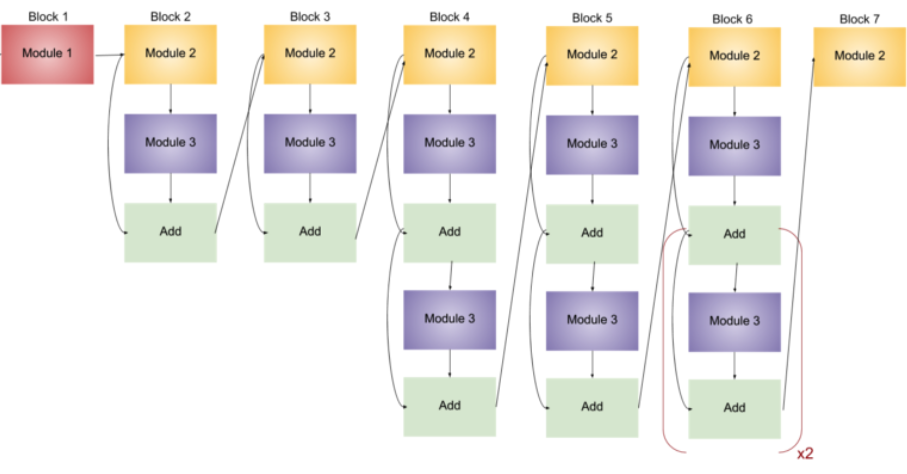
\includegraphics[width=\textwidth]{pictures/random/EfficientNetB0}
      \caption{Structure of EfficientNetB0}
      \label{fig:1}
    \end{subfigure}
    \begin{subfigure}[b]{0.49\textwidth}
      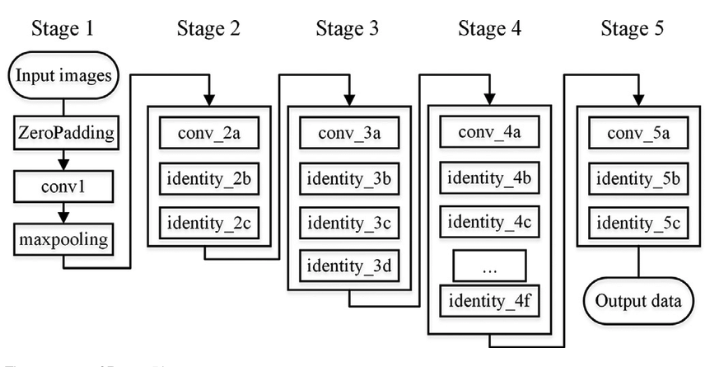
\includegraphics[width=\textwidth]{pictures/random/ResNet50structure}
      \caption{Structure of Resnet50}
      \label{fig:2}
    \end{subfigure}
    \label{fig:ArchitectureOfCNN}
\end{figure}
Throughout the experiments conducted in this study different stages of the encoder networks were fine-tuned. The amount of parameters fine-tuned ranged from the very last layer to more than half of the
parameters in both encoders. It was found that the more layers fine-tuned, the better accuracy, up to a certain point. The time consumption also increases, with the amount of parameters fine-tuned. Because this project only focused on being able to obtain in-domain CNN like accuracy for the general domain CNN, there was no goal for being time efficient. The maximum amount of parameters fine-tuned on EfficientNetB0, were $\sim$ 3 millions, out of the total amount of 4 millions, in practice this meant to train the entire stage 7, and block c and d of stage 6. The maximum amount of parameters trained on ResNet50 were $\sim$ 15 millions, out of the total amount of 23.6 millions, in practice this meant to train the entire stage 5. To achieve the best model, early stopping were introduced to measure improvements on the validation dataset. All models in the \hyperref[sec:Results]{Results} section stopped early, which suggest they all stopped at the optimal point.

\subsection{Contrastive Learning}
\begin{figure}[H]
    \centering
    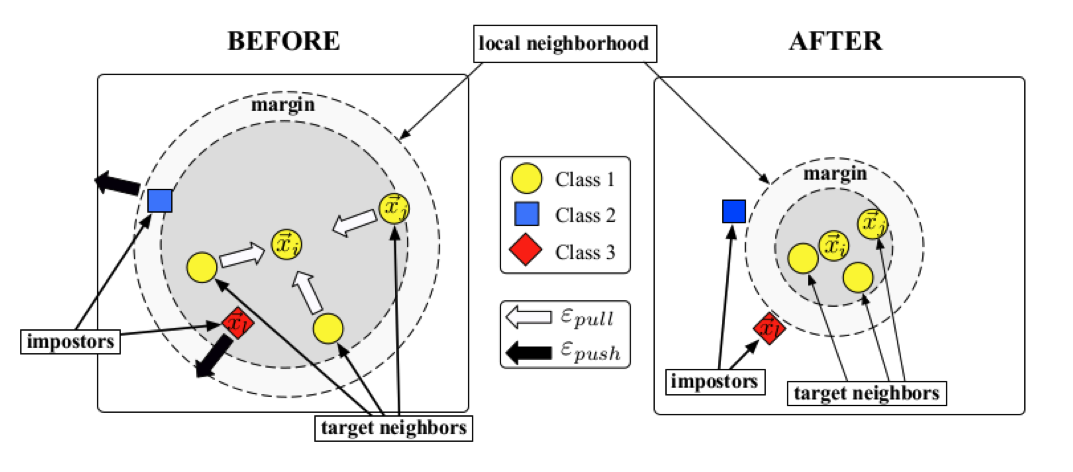
\includegraphics[width =\textwidth]{pictures/random/ContrastiveLoss}
    \caption{Crontrastive Loss in action\footnote{https://researchweb.iiit.ac.in/~praveen.krishnan/compreExam/slides/T4-DistanceMetricLearningBeyond0-1Loss.pdf}}
    \label{fig:ContrastiveLoss}
\end{figure}
The contrastive loss model implemented in this project, had the intention of binding rooms with similar labels closer together and pushing apart rooms with different labels, as seen in \autoref{fig:ContrastiveLoss}, to achieve a higher top-1 accuracy. This was done using the contrastive loss function, showcased above. The loss function takes as input the feature vectors, the image labels and a margin. As shown above, the loss function will minimise the distance between feature vectors of same class, and maximise the distance to feature vectors of different classes for all feature vectors within the margin. For the object of the project, the margin were set to 1. This number was chosen because most of the distances ranged from 0.5 to 5. The implemented method used in \textbf{\textit{Khosla}}\autocite{khosla2020supervised} did not use a pre-trained network, unlike the implementation used in this project.

\subsection{Previous Work and improvements}\label{Improvement}
A previous study by \textbf{\textit{Ingwersen}}\autocite{Ingwersen}, found that the general-domain model (ResNet50 with ImageNet) did not manage to produce meaningful representations of rooms. \textbf{\textit{Ingwersen}} made the choice of focusing on the in-domain model, which was a VGG16 model pre-trained on the Places365 dataset, as this was on the baseline level 10\% better than the general domain model. See \hyperref[appendix: A]{appendix: A}. \textbf{\textit{Ingwersen}} reported the baselines of the general-domain model to have a top-1 accuracy of 33\% when using ResNet50 preprocessing scheme. The author of this study found a problem when rerunning the baseline tests from \textbf{\textit{Ingwersen}}, the ResNet50 preprocessing scheme was used incorrectly, and therefore reported a wrong baseline top-1 accuracy for the ResNet50 model. The new improved baseline suggested that the general-domain model would perform almost as good as the in-domain VGG16 model used in \textbf{\textit{Ingwersen}}. The below table show the baseline improvements:
\begin{table}[H]
\centering
\begin{tabular}{lll}
Model and preprocessing scheme     & Improved                      & \textit{\textbf{Ingwersen}}      \\ \hline
\multicolumn{1}{|l|}{Effecientnet} & \multicolumn{1}{l|}{0.719968} & \multicolumn{1}{l|}{\textbf{NA}} \\ \hline
\multicolumn{1}{|l|}{Resnet50}     & \multicolumn{1}{l|}{0.655529} & \multicolumn{1}{l|}{0.322}       \\ \hline
\end{tabular}
\caption{Top-1 accuracy of Baseline models}
\end{table}
These baseline results should be compared to the baseline reported in \textbf{\textit{Ingwersen}}, and yields an improved baseline of $>$30\% points. This improvement suggests that when fine-tuning the general-domain model, the model should be able to compete with the trained in-domain model implemented in \textbf{\textit{Ingwersen}}. The top performing models in \textbf{\textit{Ingwersen}} is shown in \hyperref[appendix: B]{appendix: B}. The best performing model in \textbf{\textit{Ingwersen}} has a top-1 accuracy of \textbf{78.3\%}, this is called the \textbf{Gold Standard}\label{goldstandard} throughout this study, because it is what this project aim to close the gap to.

\subsection{Optimizers}
In the novel stages of the project different optimizers were tested. The 2 optimizers tested were Adam and SGD. Different learning rates were also tested. The accuracy achieved is as follows:
\begin{table}[H]
\centering
\begin{tabular}{llllll}
Optimizer\textbackslash{}LR & 0.005  & 0.001 & 0.0005 & 0.0001 & 0.00005 \\
Adam                        & 27\%   & \textbf{33}\%  & 32\%   & 32\%   & 33\%\\
SGD                         & 35,9\% & \textbf{36}\%  & 35\%   & 35\%   & NA
\end{tabular}
\caption{Top-1 Accuracy, with regards to different learning rates and optimizers.}
\end{table}
The SGD is a stochastic gradient descent optimizer, which stochastically updates parameters. SGD proved to work well with transfer learning and the problem definition of this project. Adam were investigated, because it was described in \textbf{\textit{Ingwersen}}\autocite{Ingwersen} as maybe being the better choice for that project. \textbf{\textit{Ingwersen}} trained auto encoders on top of the in-domain model, the teach the model to do better representations, and used Adadelta as the optimizer. However Adadelta is not optimal to use when transfer learning, and SGD were chosen because it outperformed Adam. The accuracies above, were measured before the preprocessing scheme were improved, and was unfortunately not revised after the improvement, why the accuracies are below the baseline results.

\subsection{Revising the Dataset}
During the experiments, different rooms were identified as being labeled wrong. Therefore the entire dataset were revised. $\sim$ 10-20\% of the living rooms and bedrooms were empty, and were removed from the dataset, because these empty rooms will not help home seekers in choosing their preferred aesthetics. This had the effect of binding images with similar labels closer together, \hyperref[appendix: E]{appendix: E}. 
The revised dataset is used to train all models in \hyperref[sec:Results]{Results}.
